%--------------------
% Packages
% -------------------
\documentclass[12pt,a4paper,titlepage]{article}
\usepackage[toc,page]{appendix}
\usepackage{amssymb, amsmath}
\usepackage[pdftex]{graphicx}
\usepackage{amsfonts} 
\usepackage{amsmath}
\usepackage[pdftex,linkcolor=black,pdfborder={0 0 0}]{hyperref}
\usepackage{calc}
\usepackage{tikz}
\usetikzlibrary{shapes.geometric, arrows}
\tikzstyle{startstop} = [rectangle, rounded corners, minimum width=3cm, minimum height=1cm,text centered, draw=black, fill=red!30]
\tikzstyle{io} = [trapezium, trapezium left angle=70, trapezium right angle=110, minimum width=3cm, minimum height=1cm, text centered, draw=black, fill=blue!30]
\tikzstyle{process} = [rectangle, minimum width=3cm, minimum height=1cm, text centered, draw=black, fill=orange!30]
\tikzstyle{decision} = [diamond, minimum width=3cm, minimum height=1cm, text centered, draw=black, fill=green!30]
\tikzstyle{arrow} = [thick,->,>=stealth]

\usepackage{enumitem}
\linespread{1.2} % Set linespace
\usepackage[a4paper, lmargin=0.1666\paperwidth, rmargin=0.1666\paperwidth, tmargin=0.1111\paperheight, bmargin=0.1111\paperheight]{geometry} %margins
\usepackage{graphicx}
\usepackage{nomencl}
\makenomenclature

\title{\Huge \underline{ Decision Theory and Design Optimisation}}
\author{Debjit Hore.}
\date{\today}
%-----------------------
% Begin document
%-----------------------
\begin{document}
\maketitle
\mbox{}
\nomenclature{\(\Omega\)}{Feasible set/region.}
\nomenclature{\(\alpha_{k}\)}{Step size.}
\nomenclature{\(\nabla\)}{Gradient.}
\nomenclature{\(g\)}{Gradient.}
\nomenclature{\(D\)}{Derivative.}
\nomenclature{\(T\)}{Tangent Space.}
\nomenclature{\(N\)}{Normal Space.}
\nomenclature{\(\lambda\)}{Lagrange Parameter.}
\nomenclature{\(\mu\)}{KKT Parameter.}
\nomenclature{\(\gamma\)}{Penalty Parameter.}
\nomenclature{\(h(x)\)}{Equality Constraint.}
\nomenclature{\(g(x)\)}{Inequality Constraint.}
\nomenclature{\(P(\textbf{\textit{x}})\)}{Penalty Function.}
\nomenclature{\(\textbf{H}\)}{Hessian.}
\nomenclature{\(\textit{\underline{d}}\)}{Feasible Direction.}

\printnomenclature

\clearpage
\tableofcontents

\clearpage
\section{Introduction}
``Mathematics is the language with which God wrote the universe"-Galileo.\\[1\baselineskip]
Optimisation is the process of maximising or minimising a desired objective function, while satisfying the prevailing constraints. Nature has infinite examples where an optimum state of the system is sought. As such the application of ``optimisation'' can be seen in nature as well as human creations. Some common examples are as follows:
{\begin{enumerate}
    \item A liquid droplet in zero gravity attaining a perfect sphere shape to minimise surface area for a given volume.
    \item Naturally occurring honeycomb structures ( which humans have effectively implemented and used ) are one of the most compact packaging arrangements.\
    \item Genetic mutation for survival is another natural optimisation process.
    \item Modern Machine Learning techniques are geared towards minimising a given `cost function' thereby minimising error.
\end{enumerate}}

\subsection{Brief history of Optimisation.}
\begin{enumerate}
    \item Euclid of Alexandria (325-265 BCE) solved early optimisation problems in geometry.
    \item Heron of Alexandria (10-75 CE) showed that light travels between points through the path of shortest length.
    \item Pappus of Alexandria (290–350 CE), among his many contributions to optimization, argued that the hexagon repeated in honeycomb is the optimal regular polygon for storing honey; its hexagonal structure uses the least material to create a lattice of cells over a plane.
    \item The use of a gradient method (requiring derivatives of the functions) for minimization was first presented by Cauchy in 1847. 
    \item Karush, Kuhn, and Tucker who derived the “KKT” optimality conditions for constrained problems [1939, 1951]. Thereafter,particularly in the 1960s, several numerical methods to solve nonlinear optimization problems were developed.
    \item Methods for unconstrained minimization include conjugate gradient methods of Fletcher and Reeves [1964] and the variable metric methods of Davidon–Fletcher–Powell (DFP) in [1959].
    \item  Rosenbrock's method of orthogonal directions [1960], simplex method of Nelder and Meade [1965]. 
    \end{enumerate}
    
%
\subsection{Flow of an Optimisation Problem.}
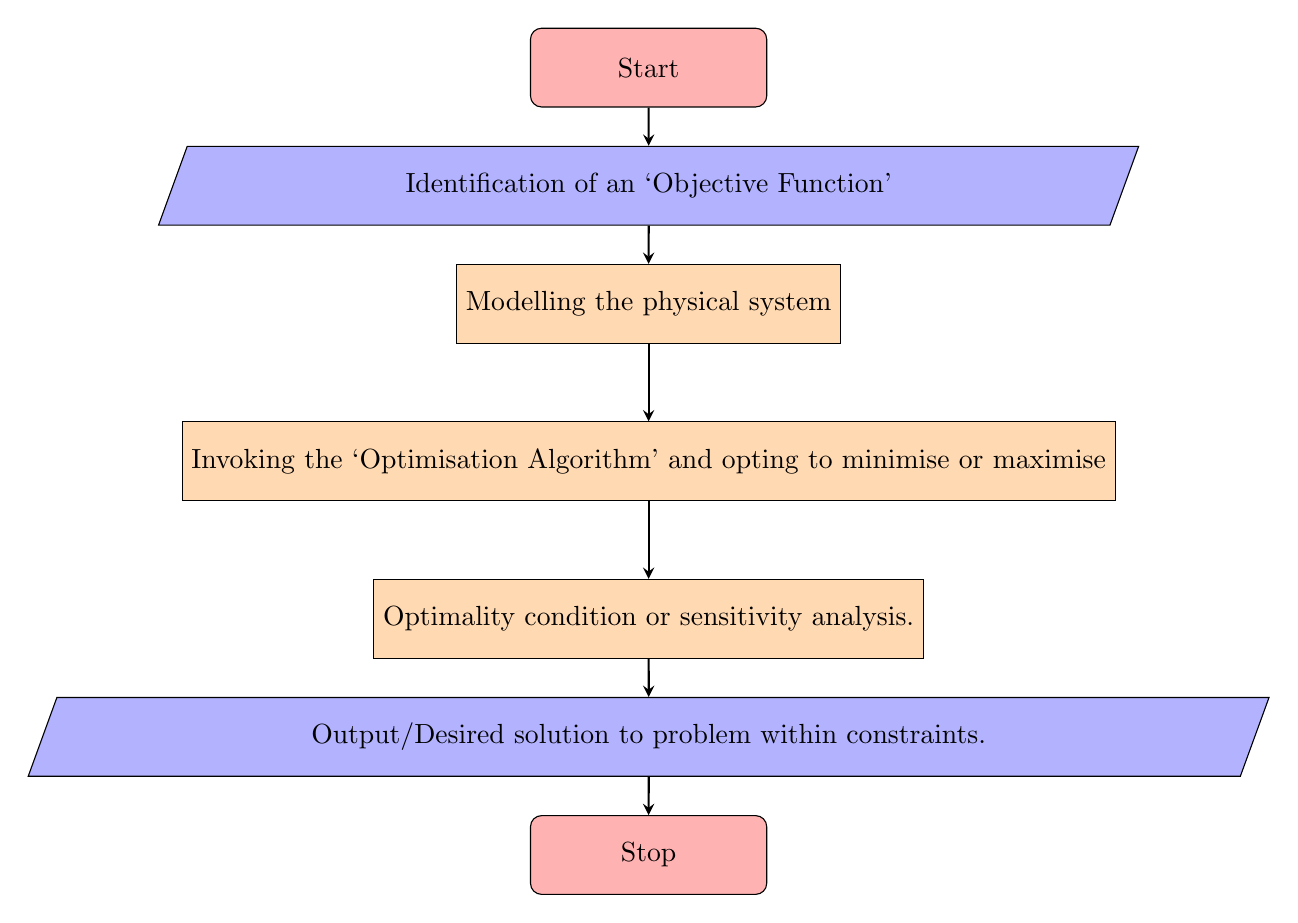
\begin{tikzpicture}[node distance=1.5 cm]
\node (start) [startstop] {Start};
\node (in1) [io, below of=start] {Identification of an `Objective Function'};
\node (pro1) [process, below of=in1] {Modelling the physical system};
\node (pro2) [process, below of=pro1, yshift=-0.5cm] {Invoking the `Optimisation Algorithm' and opting to minimise or maximise};
\node (pro3) [process, below of=pro2, yshift=-0.5cm] {Optimality condition or sensitivity analysis.};
\node (out1) [io, below of=pro3] {Output/Desired solution to problem within constraints.};
\node (stop) [startstop, below of=out1] {Stop};
\draw [arrow] (start) -- (in1);
\draw [arrow] (in1) -- (pro1);
\draw [arrow] (pro1) -- (pro2);
\draw [arrow] (pro2) -- (pro3);
\draw [arrow] (pro3) -- (out1);
\draw [arrow] (out1) -- (stop);
\end{tikzpicture}

You should add the citations as described here \cite{sadd2009elasticity}.

\subsection{Types of Problems:}
\begin{enumerate}
    \item Linear Programming.
    \item Integer Programming.
    \item 0-1 Programming.
    \item Mixed Integer Programming. (MIP)
    \item Mixed Integer Non-Linear Programming. (MINLP)
    \item Quadratic Programming.
    \item Convex Programming. (Local solution is Global solution)
    \item Combinatorial Problems.
\end{enumerate}
%

\section{Unconstrained Optimisation}

\subsection{First Order Necessary Condition.}
For unconstrained optimisation, if x* is a local minimiser, then the rate of increase of function \textbf{f} at x* in any feasible direction \textbf{\underline{d}} in the feasible region $\Omega$ is non-negative :

\begin{equation}
    \dfrac{\partial f}{\partial\underline{d} } \geq 0 \label{eq1} 
\end{equation}
For an interior point of $\Omega$ if x* is local minimiser then :
\begin{equation}
    \nabla f (x*)=  0 \label{eq2} 
\end{equation}


\subsection{Second Order Necessary Condition.}
For \textbf{SONC}, x* is a local minimiser of \textbf{f} over $\Omega$ and \textbf{\underline{d}} is a feasible direction if:

\begin{equation}
    \underline{d}^T \nabla f(x*)= 0 \label{eq3}
\end{equation}
\textbf{then}
\begin{equation}
    \underline{d}^T \textbf{H(x*)} \underline{d} \geq 0 \label{eq4}
\end{equation}
where H(x*) is the Hessian of f at x*.

\subsection{Second Order Sufficient Condition}
Suppose \textbf{\underline{f}} is a function from \textbf{$\mathbb{R}^n$ $\rightarrow$ $\mathbb{R}$} is twice differentiable such that 
\begin{equation}
    \nabla f(x*)=0    
\end{equation}
and
\begin{equation}
    \textbf{H(x*)} > 0
\end{equation}
then x* is a strict local minimiser of \textbf{f}.

\subsection{Univariate Unconstrained Optimisation.}
1D problem is defined as:
minimise(f), \textbf{f:$\mathbb{R}$ $\rightarrow$ $\mathbb{R}$} when $\Omega = \mathbb{R}$, where $\Omega$ is the domain of \textbf{f}.
The approach is to use an iterative search algorithm also called a `line-search' method. \\
\textbf{Linear Search Algorithms}: 
\begin{enumerate}
    \item Golden Section Method.
    \item Fibonacci Method.
    \item Bisection Method.
    \item Secant Method.
    \item Newton's Method
\end{enumerate}

A sample image (Fig. \ref{fig1}) shows how a typical line search algorithm works: 
\begin{figure}[h!tb]
	\centering
	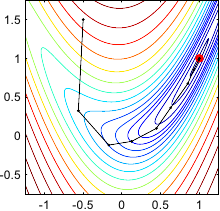
\includegraphics[scale=1]{line_searchdemo.png}
	\caption{Typical Linear Search Algorithm} \label{fig1}
\end{figure}
\\
\textbf{\underline{Unimodality}} of the objective function is an important assumption in most of these line-search algorithms, which means there is an unique x* such that \emph{f} is monotonically decreasing for x $\leq$ x* and monotonically increasing for x $\geq$ x*, which means there is a \textbf{unique} global minimum.
\subsubsection{Golden Section Method}
Target: To find argmin(\textbf{f}) over a closed interval $[a^0, b^0]$ where \textbf{f :\textbf{$\mathbb{R}$ $\rightarrow$ $\mathbb{R}$}} and a unimodal function.
\begin{enumerate}
    \item Choose $[a^1, b^1]$ such that $a^1-a^0=b^0-b^1=\rho(b^0-a^0)$
    \item If $f(a^1) < f(b^1)$ then minimiser in range $[a^0, b^1]$ else in range $[a^1,b^0]$
    \item Start with reduced range of uncertainty and repeat the process.
\end{enumerate}
Here $\rho$ is the golden ratio and equals 0.61803
\subsubsection{Fibonacci Method}
In Fibonacci, we vary the value of $\rho$ at every step, such that the updation rule is as follows:
\begin{equation}
   \rho_{k+1}= 1- \frac{\rho_{k}}{(1-\rho_{k})}
\end{equation}
\subsubsection{Bisection Method}
\begin{enumerate}
    \item For starters, $x^0$ is chosen such that $x^0=\frac{(a^0+b^0)}{2}$
    \item Evaluate $f'(x^0)$.
    \item If this value is less than 0 then x* (minimiser) lies right of $x^0$ and interval is reduced to $[x^0, b^0]$, or else $[a^0, x^0]$ 
    \item If $f'(x^0)$ =0, then x*= $x^0$, search is terminated.
\end{enumerate}
\subsubsection{Newton's Method}
\begin{enumerate}
    \item This method requires that $f'(x)$ and $f''(x)$ exist at every iteration point.
    \item In that case the next iteration point is obtained as follows:
\begin{equation}
   x_{k+1}= x_{k}-\frac{f'(x)}{f''(x)}
\end{equation}
    \end{enumerate}
\subsubsection{Secant Method}
\begin{enumerate}
    \item In order to bring down the continuity requirement needed in Newton's method for the second derivative to exist, the second derivative is approximated in Secant method as follows: 
    \begin{equation}
   x_{k+1}= x_{k}-\frac{x_{k}-x_{k-1}}{f'(x_{k})-f'(x_{k-1})}f'(x_{k})
\end{equation}
\end{enumerate}

\subsection{Multivariate Unconstrained Optimisation.}
\subsubsection{Gradient Method.}
These methods use the gradient of the function at a given point to iterate to the extremiser. To put it simply, the direction of maximum rate of increase/decrease of a real valued function at a point is orthogonal to the level set of the function through that point. \\
Fig. \ref{fig2} shows a gradient descent algorithm converging to different local minimiser depending on initial choice 
\begin{figure}[h!tb]
	\centering
	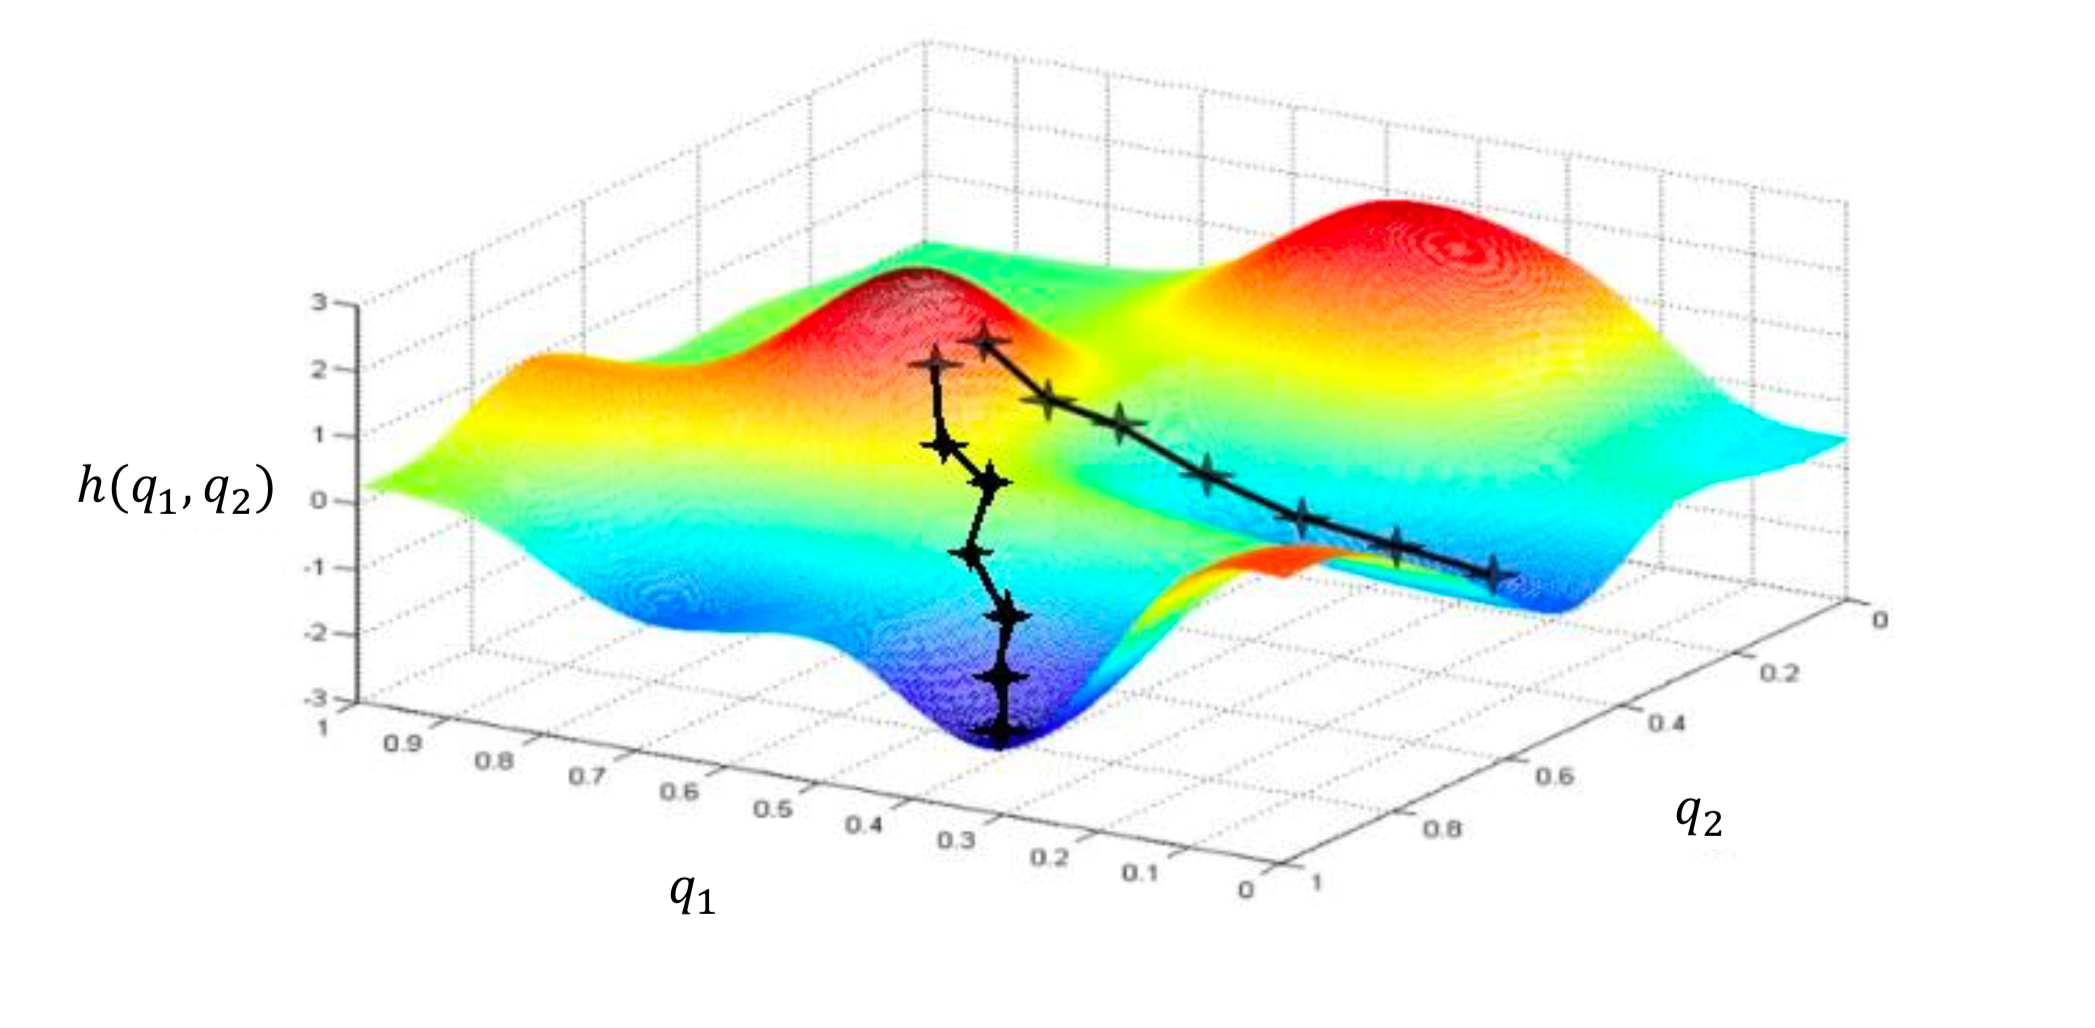
\includegraphics[scale=0.4]{gradientdescentimg.png}
	\caption{Gradient Descent Algorithm} \label{fig2}
\end{figure}
\\
\textbf{\underline{Algorithm Development.}}
\begin{equation}
    x_{k+1}= x_{k}- \alpha_{k} \nabla f(x_{k})
\end{equation}
\textbf{Method of Steepest Descent.}
This is a modification of the Gradient Algorithm where the step size $ \alpha_{k} $ is chosen to achieve maximum amount of `Objective Function' at each individual step.
\begin{equation}
    \alpha_{k}= argmin f(x_{k}-\alpha \nabla f(x_{k}))
\end{equation}
\textbf{Termination Criteria.} \\
\textbf{$\nabla f(x_{k+1})=0$} can never ideally happen so a specified thresh-hold is set. 
\begin{enumerate}
    \item Terminate if $||x||$ is less than a specified  value.
    \item Terminate if $|f(x_{k+1})- f(x_{k})| < \epsilon $ where $\epsilon$ is pre-set.
    \item Terminate if $ ||x_{k+1}-x_{k}|| < \epsilon $ where $\epsilon$ is pre-set.
\end{enumerate}

\subsubsection{Conjugate Direction Method.}
The Conjugate Direction Methods are a dramatic improvement over the steepest descent method. They can find the minimum of a quadratic function of n variables in n iterations, as contrasted to Steepest Descent Method. \\
The statement this method poses is that `For a quadratic function of \textit{n} variables $f(x)= \frac{1}{2}{x^T}\textbf{Q}x-{x^T}b$, such that $x  \epsilon  \mathbb{R}^T, Q= {Q^T} > 0$, the best direction of search is in the \textit{\textbf{Q}-conjugate direction}. Basically, two directions $d^{(1)}$ and $d^{(2)}$ in $\mathbb{R}^n$ are said to be \textit{\textbf{Q}-conjugate} if \textit{$\textbf{d}^{(1)}\textbf{Qd}^{(2)}$}=0. \\
\\\textbf{\underline{Basic Conjugate Direction Algorithm.}}
\begin{enumerate}
    \item $g^{(k)}= \nabla f(x^{(k)}= \textbf{Q}x^{(k)}-b.$
    \item $\alpha_{k}= \frac{-g^{(k)T}d^{(k)}}{d^{(k)T}Qd^{(k)}}.$
    \item $x^{(k+1)}  = x^{(k)}+ \alpha_{k}d^{(k)}$
\end{enumerate}
In the conjugate direction algorithm another important relationship that holds true throughout is $ \textbf{g}^{(k+1)T}\textbf{d}^{(i)}$=0 for all k, $0 \leq k \leq n-1$, and 0 $\leq i \leq k $.\\
The conjugate direction algorithm:
\begin{enumerate}
    \item Solves quadratics of n variables in n steps.
    \item Requires no Hessian matrix evaluation or inversion, and no storage of matrix is required.
\end{enumerate}

\subsubsection{Conjugate Gradient Algorithm}
Instead of making use of pre-specified conjugate directions, CGA computes the directions as the algorithm progresses. At every iteration, direction is calculated as linear combination of previous direction and current gradient, making sure that the directions are mutually \textit{\textbf{Q}-conjugate}.\\The Conjugate Gradient Algorithm proceeds as follows: 
\begin{enumerate}
    \item Set k:=0, select initial point $x^{(0)}$
    \item $g^{(0)}= \nabla f(x^{(0)}. $ If $g^{(0)} = 0$ stop; else $d^{(0)}= -g^{(0)}$
    \item $\alpha_{k}= \frac{-g^{(k)T}d^{(k)}}{d^{(k)T}Qd^{(k)}}.$
    \item $x^{(k+1)}  = x^{(k)}+ \alpha_{k}d^{(k)}$
    \item $g^{(k+1)}= \nabla f(x^{(k+1)}.$ If $g^{(k+1)}=0$; STOP
    \item $\beta_{k}= \frac{-g^{(k+1)T}Qd^{(k)}}{d^{(k)T}Qd^{(k)}}.$
    \item $d^{(k+1)}= -g^{(k+1)}+\beta_{k}d^{(k)} $
    \item Set k=k+1; go to STEP 3.
\end{enumerate}
The conjugate gradient algorithm for \textbf{non-quadratic function} optimisation uses different updation criteria for $\beta_{k}$. These include:
\\ The \textbf{Hestenes-Stiefel Formula}:
\begin{equation}
    \beta_{k}= \frac{g^{(k+1)T}[g^{(k+1)}-g{(k)}]}{d^{(k)T}[g^{(k+1)}-g{(k)}]}
\end{equation}
The \textbf{Polak-Ribiere Formula}:
\begin{equation}
    \beta_{k}= \frac{g^{(k+1)T}[g^{(k+1)}-g{(k)}]}{[g^{(k)T}g{(k)}]}
\end{equation}
The \textbf{Fletcher-Reeves Formula}:
\begin{equation}
        \beta_{k}= \frac{g^{(k+1)T}g^{(k+1)}}{[g^{(k)T}g{(k)}]}
\end{equation}
\subsubsection{Newton's Method}
This method uses a quadratic approximation of the objective function and then minimises the approximate (quadratic) function instead of original objective function. If original function is not quadratic then this method will provide only an estimate of the position of the true minimiser. The Newton's formula states that the approximated objective function achieves a minimum at:
\begin{equation}
    \textbf{x}^{(k+1)}= \textbf{x}^{(k)}- \textbf{H}(x^{(k)})^{-1}\textbf{g}^{(k)}
\end{equation}
There are a few drawbacks to Newton's Method:
\begin{enumerate}
    \item If the initial guess is far away from original answer then it might not give descent at consecutive iterations.
    \item Evaluation and storage of inverse of the Hessian for large dimensions is a computationally expensive process in terms of time and space complexity.
    \item The Hessian matrix needs to be positive at every step, in which case search direction may not necessarily be in direction of descent.
\end{enumerate}
To overcome this the \textbf{Levenberg-Marquardt Modification} uses a simple technique to ensure search direction is in descent direction. The expression: 
\begin{equation}
    \textbf{x}^{(k+1)}= \textbf{x}^{(k)}- (\textbf{H}(x^{(k)})+\mu_{k}\textbf{I})^{-1}\textbf{g}^{(k)}
\end{equation}
If the choice of $\mu$ is sufficiently large then all eigen values of the modified matrix are positive and the inverse of Hessian is ensured to be positive definite.
\subsubsection{Quasi-Newton Method}
To avoid the computation of the inverse Hessian as in the Newton's Method approach, the Quasi Newton method uses an approximation in place of true inverse. The approximation is updated at every stage so it exhibits some properties of the inverse.\\ The first property that the approximate inverse should have is 
\begin{equation}
    \textbf{g}^{(k)T}\textbf{H}_{k}\textbf{g}^{(k)} >0
\end{equation}
Here $\textbf{H}_{k}$ is the approximation of the inverse Hessian which should be positive definite to satisfy above relationship. Another requirement that is imposed on the approximate Hessian is 
\begin{equation}
    \textbf{H}_{k+1}\Delta \textbf{g}^{(i)}= \Delta \textbf{x}^{(i)}, 0 \leq i \leq k
\end{equation}
Keeping this consideration in mind the basic statement of Quasi Newton is presented as 
\begin{equation}
    \textbf{d}^{(k)}= - \textbf{H}_{k}\textbf{g}^{(k)},
\end{equation}
\begin{equation}
    \alpha_{k}= argmin \textbf{f}(\textbf{x}+\alpha \textbf{d}^{(k)}),
\end{equation}
\begin{equation}
    \textbf{x}^{(k+1)}= \textbf{x}^{(k)}+\alpha_{k}\textbf{d}^{(k)},
\end{equation}
The updation formulae for $\textbf{H}^{(k+1)}$ from $\textbf{H}^{(k)}$ comes in three different flavours. \\
\\ \textbf{\underline{Rank 1 Algorithm.}}
\begin{equation}
    \textbf{H}_{k+1}= \textbf{H}_{k}+ \frac{(\Delta \textbf{x}^{(k)}-\textbf{H}_{k}\Delta\textbf{g}^{(k)})(\Delta \textbf{x}^{(k)}-\textbf{H}_{k}\Delta\textbf{g}^{(k)})^T}{\Delta \textbf{g}^{(k)T}(\Delta \textbf{x}^{(k)}-\textbf{H}_{k}\Delta\textbf{g}^{(k)})}
\end{equation}
\textbf{\underline{DFP Algorithm.}}
\begin{equation}
        \textbf{H}_{k+1}= \textbf{H}_{k}+\frac{\Delta\textbf{x}^{(k)}\Delta\textbf{x}^{(k)T}}{\Delta\textbf{x}^{(k)T}\Delta\textbf{g}^{(k)}}-\frac{[\textbf{H}_{k}\Delta\textbf{g}^{(k)}][\textbf{H}_{k}\Delta\textbf{g}^{(k)}]^{T}}{\Delta \textbf{g}^{(k)T}\textbf{H}_{k}\Delta\textbf{g}^{(k)}}
\end{equation}
\textbf{\underline{BFGS Algorithm.}}
\begin{equation}
    \textbf{H}_{k+1}= \textbf{H}_{k}+ (1+\frac{\Delta \textbf{g}^{(k)T}\textbf{H}_{k}\Delta\textbf{g}^{(k)}}{\Delta\textbf{g}^{(k)T}\Delta\textbf{x}^{(k)}})\frac{\Delta\textbf{x}^{(k)}\Delta\textbf{x}^{(k)T}}{\Delta\textbf{x}^{(k)T}\Delta\textbf{g}^{(k)}} - \frac{(\textbf{H}_{k}\Delta\textbf{g}^{(k)}\Delta\textbf{x}^{(k)T})+(\textbf{H}_{k}\Delta\textbf{g}^{(k)}\Delta\textbf{x}^{(k)T})^{T}}{\Delta\textbf{g}^{(k)T}\Delta\textbf{x}^{(k)}}
\end{equation}

\section{Non-Linear Constrained Optimisation}
In addition to an objective function, a constrained optimisation problem has constraints imposed on the solution that can be in the form of equality or inequality constraints, and any points satisfying these constraints is termed as a feasible point. Collection of all such feasible points is called a feasible set. When the constraints are linear it is called a linear constrained optimisation problem or non-linear. If we have an `\textit{n}' dimensional function and `\textit{m}' constraints then the solution set will lie on a (n-m) dimensional surface.\\[1\baselineskip]
\textbf{\underline{Regular Point}}: A point $\textbf{x}^{*}$ satisying the constraints is called a `\textbf{Regular Point}' if all columns of the Jacobian matrix of the constraints are linearly independent.\\
\textbf{\underline{Tangent Space}} :In mathematics, the tangent space of a manifold generalizes to higher dimensions the notion of tangent planes to surfaces in three dimensions and tangent lines to curves in two dimensions. In the context of physics the tangent space to a manifold at a point can be viewed as the space of possible velocities for a particle moving on the manifold. The tangent space at a point $\textbf{x}^{*}$ on the surface $\textbf{S}= [\textbf{x}\epsilon \mathbb{R}^{n} | \textbf{h}(x)=0]$ where h $\epsilon$ $C^{1}$ is the set
\begin{equation}
    T(x^{*})= [\underline{y} | Dh(\underline{x}^{*})\textbf{\underline{y}}]= 0
\end{equation}
\textbf{\underline{Normal Space}} : Normal space $N(x^{*})$ at a point $x^{*}$ on surface \textbf{S} is the set
\begin{equation}
    N(x^{*})= [\underline{x} \epsilon \mathbb{R}^{n} | \underline{x} = Dh(\underline{x}^{*})^{T}\underline{z}, z \epsilon \mathbb{R}^{n}]
\end{equation}
It is orthogonal to the Tangent Space.
\subsection{Lagrange Theorem:}
For n=2 and m=1, if point $x^{*}$ is a minimiser of \textbf{f}: $\mathbb{R}^{2}\rightarrow\mathbb{R}$ subjected to constraint h(\underline{x} )=0, then $\nabla f (x^{*})$ and $\nabla h(\underline{x}^{*})$  are parallel and there exists a scalar $\lambda ^{*}$ such that
\begin{equation}
    \nabla f(\underline{x}^{*})+ \lambda^{*} \nabla h(\underline{x}^{*}) = 0
\end{equation}
$\lambda^{*}$ is called the `Lagrange Multiplier'. Lagrange Theorem provides a \textbf{first order necessary condition} for a point to be a local minimiser and also converts a constrained optimisation problem to an unconstrained one. This is a necessary but not sufficient condition.\\
The \textbf{second order necessary condition} is as follows:
\begin{equation}
    \underline{y}^{T}\textbf{H}_{l}(\underline{x}^{*}, \underline{\lambda})\underline{y} \geq 0 
\end{equation}
For all \underline{y} $\epsilon$ T$(\underline{x}^{*})$. $\textbf{H}_{l}(\underline{x}^{*}, \underline{\lambda})$ is the Hessian of the Lagrangian function.\\
The \textbf{second order sufficient condition} along the same lines:
\begin{equation}
    \underline{y}^{T}\textbf{H}_{l}(\underline{x}^{*}, \underline{\lambda})\underline{y} > 0 
\end{equation}
For all \underline{y} $\epsilon$ T$(\underline{x}^{*})$. $x^{*}$
is a strict local minimiser of objective function \textbf{\textit{f}}.

\subsection{Karush–Kuhn–Tucker Algorithm}
Lagrange method for Constrained Optimisation problems could handle only equality constraints in the problem statement. \textbf{KKT} algorithm, on the other hand helps us tackle a mixed set of constraints with both equality and inequality constraints. We take into consideration problems that look like
\begin{center}
    minimise \textit{f(\textbf{x})}\\
    subject to \textit{\textbf{h(x)}}=0,\\
    \hspace{1.90 cm} \textit{\textbf{g(x)}} $\leq$ 0,
\end{center}
where f: $\mathbb{R}^{n}\rightarrow\mathbb{R}$, h: $\mathbb{R}^{n}\rightarrow\mathbb{R}^{m}$, m $\leq$ n, g: $\mathbb{R}^{n}\rightarrow\mathbb{R}^{p}$. This is the general convention adopted for any problem.\\[1\baselineskip]
\textbf{\underline{Active and Inactive Constraints.}}\\
An inequality constraint is said to be \textit{active} at $x^{*}$ if $g_{j}(x^{*})$=0 and is said to be \textit{inactive} if $g_{j}(x^{*}) < 0$ \\
The KKT Theorem states that if $x^{*}$ is a regular point which is a local minimiser for f subjected to \textit{\textbf{h(x)=0}}, \textit{\textbf{g(x)}} $\leq$ 0, then there exists a $\boldsymbol{\lambda^{*}}$ and $\boldsymbol{\mu^{*}}$ such that:
\begin{enumerate}
    \item $\boldsymbol{\mu}^{*} \geq 0$
    \item $ Df(\boldsymbol{x}^{*})+ \boldsymbol{\lambda}^{*T}D\boldsymbol{h(x^{*})} + \boldsymbol{\mu}^{*T}D\boldsymbol{g(x^{*})} = 0^{T}$
    \item $\boldsymbol{\mu}^{*T}\boldsymbol{g(x^{*})} = 0$
    \item $\boldsymbol{h(x^{*})}=0$
    \item $\boldsymbol{g(x^{*})} \leq 0$
\end{enumerate}
The \textbf{FONC} and \textbf{SONC} are similar to the Lagrange Theorem where the \textit{Gradient} of the modified function is equated to 0, and the \textit{Hessian} of the modified function is tested for positive definiteness using vectors from the tangent space of the equality and inequality constraints. 
\subsection{Penalty Methods.}
This is another method of converting a Constrained Optimisation problem to an Unconstrained Optimisation problem of the form 
\begin{center}
    minimise $f(\boldsymbol{x})+\gamma P(\boldsymbol{x}),$
\end{center}
where $\gamma$ $\epsilon$ $\mathbb{R}$ is a positive constant called the \textit{penalty parameter} and P: $\mathbb{R}^{n} \rightarrow \mathbb{R}$ is the \textit{penalty function}. The requirements for choosing the Penalty Function is as follows:
\begin{enumerate}
    \item \textit{P} is continuous.
    \item \textit{P(\textbf{x})} $\geq$ 0, for all x $\epsilon$ $\mathbb{R}^{n}$
    \item \textit{P(\textbf{x})} = 0 iff x $\epsilon$ $\Omega$ i.e. x is feasible. 
\end{enumerate}
Clearly, for the unconstrained problem above to be a good approximation to the original problem, the penalty function P must be chosen appropriately. The role of the penalty function is to``penalize" points that are outside the feasible set.
We would expect that the larger the value of the penalty parameter $\gamma$, the closer the approximated solution will be to the true solution, because points that violate  the constraints are penalized more heavily.

%
%
\clearpage
\bibliographystyle{unsrt}
\bibliography{sample}
\end{document}